\section{Технологическая часть}

\subsection{Выбор языка программирования}
В качестве языка программирования был выбран С \cite{c}. Для сборки модуля использовалась утилита make.

Была выбрана среда разработки Visual Studio Code \cite{VStudio}, так как она бесплатная, кроссплатформенная,  а также позволяет использовать все возможности консоли, не переключаясь между окнами. \newline

\subsection{Структура загружаемого модуля}
Реализованный модуль включает в себя следующие функции:
\begin{itemize}
	\item \textbf{fw\_init()} -- функция инициализации модуля;
	
	\item \textbf{fw\_exit()}-- функция выгрузки модуля;
	
	\item \textbf{hide()} -- функция изменения видимости модуля (скрытие);
	
	\item \textbf{unhide()} -- функция изменения видимости модуля (обнаружение);
	
	\item \textbf{fw\_read(struct file *filp, char \_\_user *buff, size\_t count, loff\_t *f\_pos)} -- функция чтения, описываемая в структуре struct file\_operations;
	
	\item \textbf{fw\_write(struct file *filp, const char \_\_user *buff, size\_t count, loff\_t *f\_pos)} -- функция записи, описываемая в структуре struct file\_operations;
	
	\item \textbf{add\_rule(struct fw\_rule *rule)} -- добавление нового правила;
	
	\item \textbf{del\_rule(struct fw\_rule *rule)} -- удаление правила;
	
	\item \textbf{fw\_in\_filter(void *priv, struct sk\_buff *skb, const struct nf\_hook\_state *state)} -- <<обёртка>> функции фильтрации для входящих пакетов;
	
	\item \textbf{fw\_out\_filter(void *priv, struct sk\_buff *skb, const struct nf\_hook\_state *state)} -- <<обёртка>> функции фильтрации для исходящих пакетов;
	
	\item \textbf{filter(void *priv, struct sk\_buff *skb, const struct nf\_hook\_state *state,
	struct list\_head *list\_rule)} -- основная функция фильтрации пакетов;
	
	\item \textbf{str\_rule(struct fw\_rule *rule)} -- функция преобразования правила фильтрации в удобный для восприятия человеком вид;
	
	\item \textbf{str\_packet(uint32\_t src\_ip, uint16\_t src\_port,uint32\_t dest\_ip, uint16\_t \, dest\_port, char *protocol\_str)} -- функция преобразования информации о перехваченном пакете в удобный для восприятия человеком вид.
\end{itemize}
%
Были также определены структуры:
%
\begin{itemize}
	\item struct file\_operations;
	
	\item struct miscdevice;
	
	\item struct nf\_hook\_ops. \newline
\end{itemize}

\subsection{Структура проекта}
Проект состоит из нескольких частей:
\begin{itemize}
	\item \textbf{fw\_module.c} -- загружаемый модуль;
	
	\item \textbf{fw.h} -- основные структуры;
	
	\item \textbf{fw.c} -- непосредственное взаимодействие с пользователем, включающее обработку вводимых им данных;
	 
	\item \textbf{errors.h} -- коды обрабатываемых ошибок.
\end{itemize}
%
В Приложении А представлены листинги каждой из частей проекта. \newline
%

\subsection{Сборка и запуск модуля}
Сборка модуля осуществляется командой make. На Листинге \ref{lst:make} приведено содержимое Makefile.

\begin{lstlisting}[caption = {Makefile}, label=lst:make]
obj-m += fw_module.o

all: fw.o fw_module.o

fw.o: fw.c fw.h
	gcc -o fw.o fw.c	

fw_module.o: fw_module.c
	make -C /lib/modules/$(shell uname -r)/build M=$(PWD) modules

clean:
	rm -rf fw *.o
	make -C /lib/modules/$(shell uname -r)/build M=$(PWD) clean
\end{lstlisting}

Для того, чтобы загрузить модуль, нужно воспользоваться командой \textbf{sudo insmod fw\_module.ko}, для того, чтобы выгрузить -- \textbf{sudo rmmod fw\_module}. \newline

\subsection{Демонстрация работы модуля} 

\subsubsection{Команды и формат задания правил}
Для того, чтобы посмотреть все команды и формат задаваемых правил, необходимо вызвать \textbf{help}. На Рисунке \ref{fig11:image} представлен результат.

\begin{figure}[h]
	\begin{center}
		{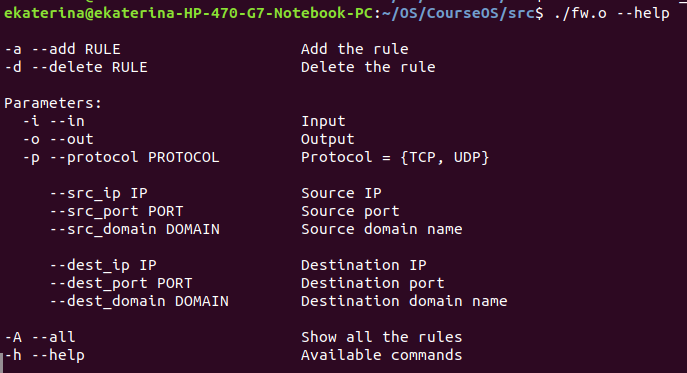
\includegraphics[scale = 0.6]{img/screenshots/help/help.png}}
		\caption{Вызов команды help}
		\label{fig11:image}
	\end{center}
\end{figure}
Для того, чтобы корректно задать правило фильтрации, необходимо соблюдать следующий формат.
\begin{enumerate}
	\item Обязательным является указание действий: добавление (add) или удаление (del).
	
	\item Также в обязательном порядке следует конкретизировать направление пакетов: входящие (in) или исходящие (out).

	\item Далее указываются основные признаки фильтрации (один или несколько):
	\begin{itemize}
		\item протокол (TCP/UDP);
		
		\item IP-адрес (источника/назначения);
		
		\item порт (источника/назначения);
		
		\item доменное имя (источника/назначения). \newline
	\end{itemize}
	
\end{enumerate}

\subsubsection{Видимость модуля}
Для скрытия модуля следует вызвать команду \textbf{hide}, а для обратного действия \textbf{unhide}. На Рисунках \ref{fig12:image} -- \ref{fig13:image} демонстрируется следующее:
\begin{enumerate}
	\item модуль загружен и виден в системе;
	
	\item вызвана команда hide;
	
	\item модуль не отображается при вызове команды lsmod;
	
	\item вызвана команда unhide;
	
	\item модуль обнаруживается при вызове команды lsmod.
\end{enumerate}

\begin{figure}[h]
	\begin{center}
		{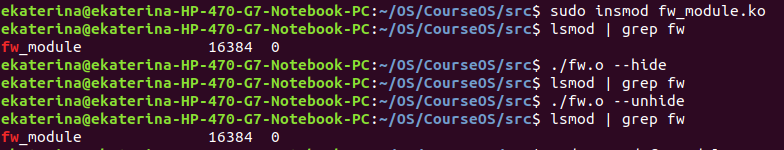
\includegraphics[scale = 0.6]{img/screenshots/hide_unhide/hide_comm.png}}
		\caption{Порядок действий}
		\label{fig12:image}
	\end{center}
\end{figure}

\begin{figure}[h]
	\begin{center}
		{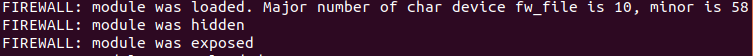
\includegraphics[scale = 0.7]{img/screenshots/hide_unhide/hide_result.png}}
		\caption{Логи}
		\label{fig13:image}
	\end{center}
\end{figure}

\subsubsection{Фильтрация по протоколу}
Для наглядности было добавлено правило, блокирующее все входящие пакеты, для передачи которых используется протокол TCP.

До того, как правило было добавлено, наблюдалась следующая динамика (Рисунок \ref{fig15:image}): происходил активный обмен пакетами, ошибки в процессе были, но не значительные.
\begin{figure}[h]
	\begin{center}
		{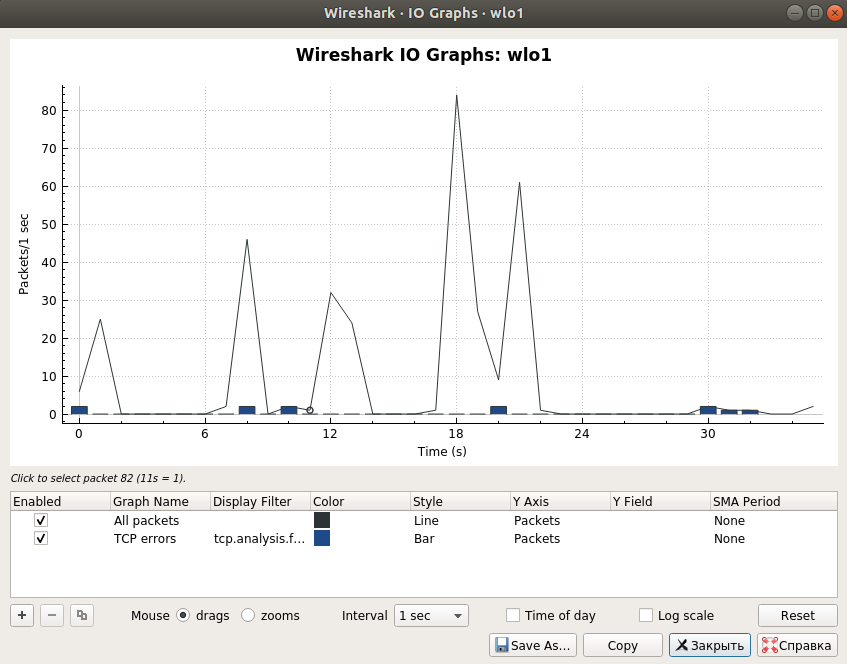
\includegraphics[scale = 0.5]{img/screenshots/rule_protocol/1_rule_protocol.png}}
		\caption{До добавления правила фильтрации}
		\label{fig15:image}
	\end{center}
\end{figure}

Когда же правило было зарегистрировано, ситуация изменилась (Рисунок \ref{fig16:image}). Примерно с 50 секунды наблюдается увеличение непринятых пакетов, более детальную информацию о них можно получить из log-файла (Рисунок \ref{fig17:image}). Легко заметить, что общее у всех непринятых пакетов -- поле протокола. 
\begin{figure}[h]
	\begin{center}
		{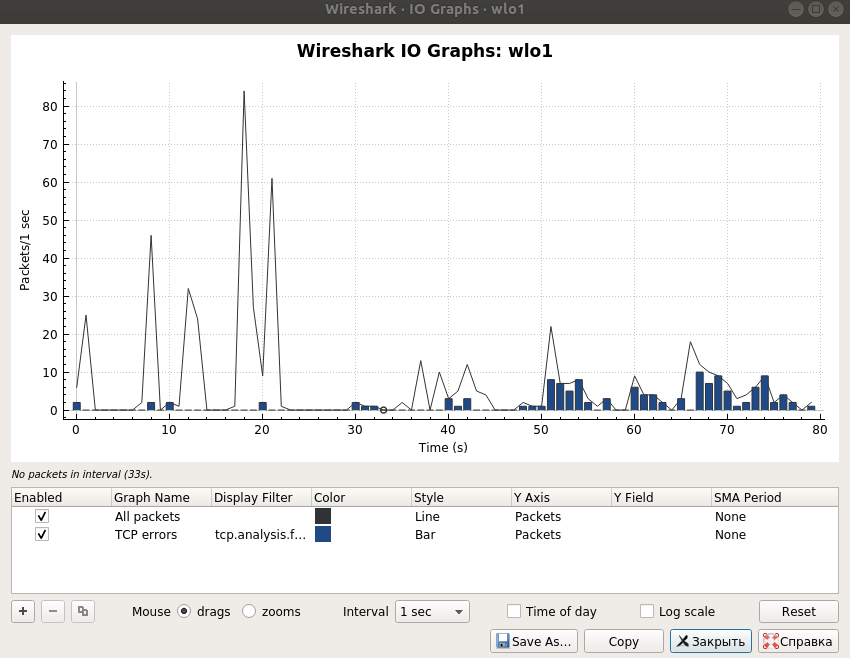
\includegraphics[scale = 0.5]{img/screenshots/rule_protocol/2_rule_protocol.png}}
		\caption{После добавления правила фильтрации}
		\label{fig16:image}
	\end{center}
\end{figure}

\begin{figure}[h]
	\begin{center}
		{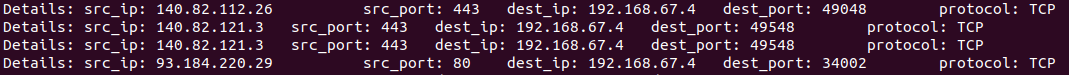
\includegraphics[scale = 0.6]{img/screenshots/rule_protocol/log_drop_packets.png}}
		\caption{Подробная информация о заблокированных пакетах}
		\label{fig17:image}
	\end{center}
\end{figure}

\newpage

При удалении правила, пакеты больше не блокируются, и это видно на Рисунке \ref{fig18:image}.
\begin{figure}[h!]
	\begin{center}
		{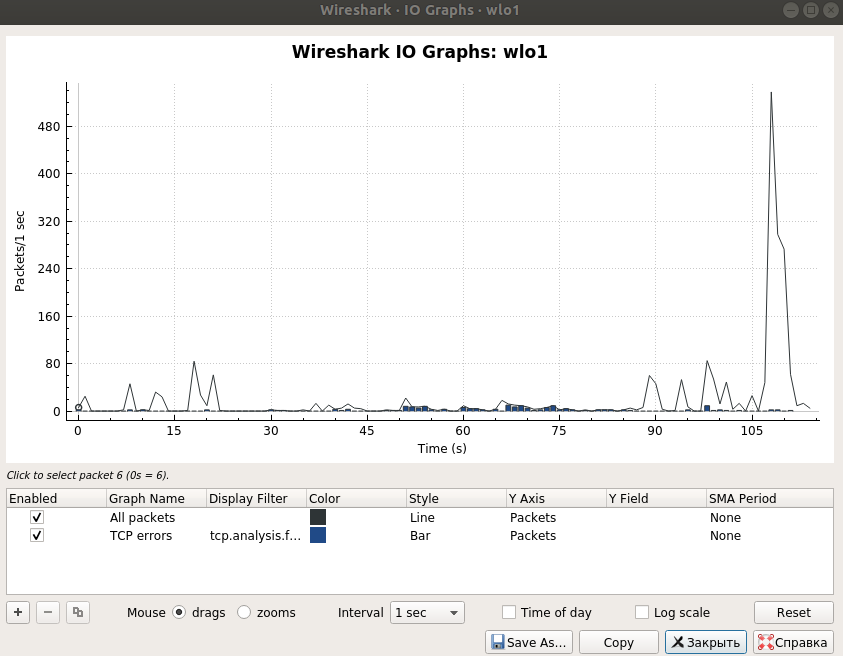
\includegraphics[scale = 0.5]{img/screenshots/rule_protocol/3_rule_protocol.png}}
		\caption{После удаления правила фильтрации}
		\label{fig18:image}
	\end{center}
\end{figure}

\newpage

С 80 секунды наблюдается резкое уменьшение ошибок и увеличение успешно обработанных пакетов. \newline

\subsubsection{Фильтрация по IP-адресу}
Модуль также предоставляет возможность отбора пакетов по IP-адресу получателя (в случае исходящих пакетов) и отправителя (входящие). 

Было добавлено следующее правило (Рисунок \ref{fig19:image}) и через некоторое время удалено (Рисунок \ref{fig20:image}). 

\begin{figure}[h]
	\begin{center}
		{
\includegraphics[scale = 0.6]{img/screenshots/ip/add_rule.png}}
		\caption{Добавление правила фильтрации по IP-адресу}
		\label{fig19:image}
	\end{center}
\end{figure}

\begin{figure}[h]
	\begin{center}
		{
\includegraphics[scale = 0.6]{img/screenshots/ip/del_rule.png}}
		\caption{Удаление правила фильтрации по IP-адресу}
		\label{fig20:image}
	\end{center}
\end{figure}

\newpage

Устройство, имеющее IP-адрес 192.168.67.132, и устройство, на котором работает межсетевой экран находятся в одной подсети. Поэтому можно с помощью команды \textbf{ping} проверить соединение.

Рисунок \ref{fig21:image} -- результат. Первые 5 и последние 6 пакетов успешно были отправлены в силу того, что правило ещё не было задано или уже удалено на момент их отправки.
\begin{figure}[h]
	\begin{center}
		{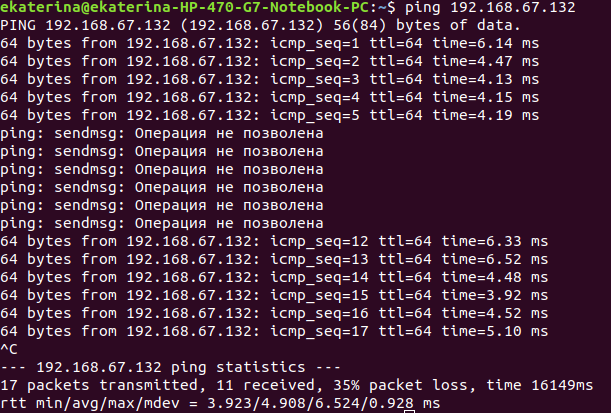
\includegraphics[scale = 0.5]{img/screenshots/ip/result.png}}
		\caption{Результат}
		\label{fig21:image}
	\end{center}
\end{figure}

\subsection{Выводы}
В этом разделе был выбран язык программирования и среда разработки, описана общая структура модуля и продемонстрированы некоторые его возможности.